\part{Cifrari storici}
\chapter{Introduzione}
I cifrari sono nati per comunicazioni "sicure" ristrette a poche persone: la cosa si contrappone alla crittografia moderna e di massa, dove la sicurezza non è più legata alla non conoscenza dell'algoritmo da parte del crittoanalista. (quindi in piena contrapposizione alla crittografia moderna di massa). Distinguiamo i seguenti tipi di cifrari:
\begin{itemize}
	\item cifrari a sostituzione, che possono essere monoalfabetici o polialfabetici;
	\item cifrari a trasposizione.
\end{itemize}
Vedremo alla fine la crittoanalisi statistica, utilizzata per forzare questi cifrari.
\section{Principi di Ruggero Bacone} 
Tutti i cifrari storici rispettano i principi di \emph{Ruggero Bacone} che dicono:
\begin{itemize}
    \item cifratura e decifratura (funzioni C e D) devono essere eseguibili facilmente;
    \item deve essere impossibile decifrare il messaggio senza conoscere l'algoritmo (non posso ricavare la funzione D se la funzione C non è nota);
    \item il crittogramma deve apparire innocente (non deve destare sospetto, deve sembrare un messaggio in chiaro).
\end{itemize}

\chapter{Cifrari a sostituzione}
\section{Tipologie}
I cifrari a sostituzione si dividono in due classi:
\begin{itemize}
	\item \textbf{monoalfabetici}, un carattere si sostituisce sempre con lo stesso carattere (per esempio il cifrario di Cesare);
	\begin{itemize}
		\item Possibile impiegare funzioni di cifratura e decifrazione più complesse dell'addizione e della sottrazione in modulo.
		\item Lo spazio delle chiavi è molto più ampio.
		\item La sicurezza è comunque molto modesta.
	\end{itemize} 
	\item \textbf{polialfabetici}, un carattere si sostituisce con una lettera scelta da un insieme di lettere possibili, secondo una qualche regola (a seconda del contesto in cui appare la lettera).
\end{itemize}
\section{Cifrario monoalfabetico: \emph{cifrario di Cesare}}
Il cifrario di Cesare è il primo di concezione moderna, tuttavia è senza chiave. La sua sicurezza si basa sulla ristrettezza di chi lo conosce. Si può generalizzare scegliendo un $k$ arbitrario che indica di quanti posti dobbiamo ruotare l'alfabeto. Supponiamo $k=3$, otteniamo
\begin{center}
	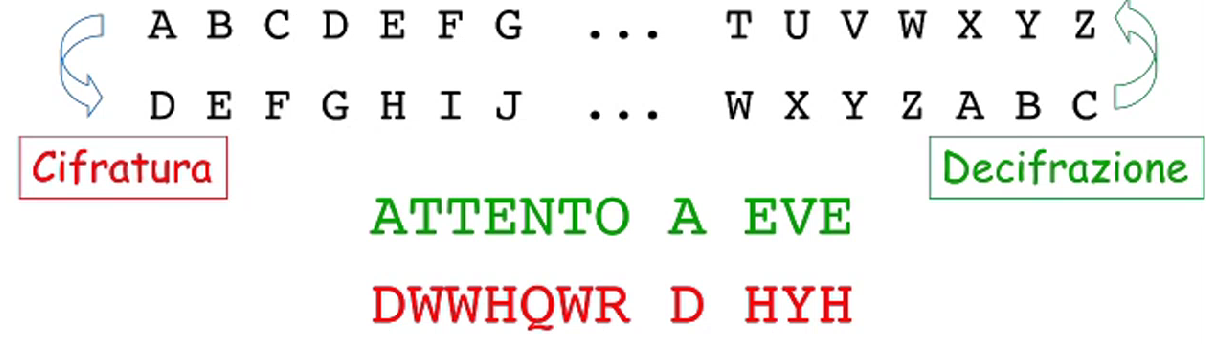
\includegraphics[scale=.45]{images/7.PNG}
\end{center}
Si legge da sopra a sotto per cifrare, da sotto a sopra per decifrare. 
\paragraph{Rafforzamento del cifrario} Possiamo rafforzare il cifrario ponendo $k$ come chiave: i due interlocutori decidono un valore $1 \leq k \leq 25$ (non $26$, altrimenti il messaggio risultante è lo stesso posto in input).
\paragraph{Generalizzazione} Indichiamo con $pos(x)$ la posizione di $x$ nell'alfabeto
\[\text{pos}(A)=0,\dots,\text{pos}(Z)=25\]
per cifrare si deve quindi sostituire $x$ con:
$$ y : \text{pos}(y) = \left(\text{pos}(x) + k\right) \text{ mod } 26 $$
dove $k$ è la chiave, $1\leq k \leq 25$. Per decifrare si sostituisce $y$ con:
$$ x : \text{pos}(x) = \left(\text{pos}(y) - k\right) \text{ mod } 26 $$Si può forzare facilmente (con attacco forza bruta) in quanto le chiavi sono poche. 
%\paragraph{Cifrario di sostituzione} Questo cifrario appartiene alla classe dei \emph{cifrari a sostituzione} cioè quelli in cui ogni lettera viene scambiata con un'altra o più di una seguendo un determinato ordine.
\paragraph{Esempio} Prendiamo $k=10$. Vogliamo cifrare $R$
\[\text{pos}(R)=17 \Longrightarrow (17+10)\,\text{mod}\,26=1=\text{pos}(B)\]
\begin{framed}
 \noindent \textbf{Esercizio da esame}, Decifrare il seguente crittogramma
	\begin{verbatim}YMNXJCJWHNXJNXJFXD\end{verbatim}
Deve essere trovata la chiave, facendo prove si trova che $k=5$ (ho usato un sito online)
\begin{verbatim}
	YMNXJCJWHNXJNXJFXD -> THISEXERCISEISEASY
\end{verbatim}
\end{framed}
\paragraph{Proprietà commutativa del cifrario} 
Questo cifrario gode della proprietà commutativa, cioè data una sequenza di chiavi e di cifrature cambiando l'ordine in cui le eseguiamo non si varia il crittogramma finale. Questo significa che
\begin{align*}
	C(C(s, k_2), k_1) = C(s, k_1 + k_2)\\
	D(D(s, k_2), k_1) = D(s, k_1 + k_2)
\end{align*}
Comporre più cifrature non aumenta la sicurezza del sistema!



\section{Cifrario monoalfabetico: \emph{cifrario affine}}
Una lettera in chiaro $x$ viene sostituita con la lettera cifrata $y$ che occupa nell'alfabeto la seguente posizione:
$$x: \text{pos}\left(y\right) = \left(a \cdot \text{pos}\left(x\right) + b\right)\text{ mod } 26 $$
Abbiamo come chiave segreta del cifrario $K = <a, b>$. Mentre la cifratura rimane cosa semplice la decifrazione diventa più complessa. 
$$ y \xrightarrow{} x : pos\left(x\right) = a^{-1} \cdot (pos\left(y\right) - b) \text{ mod } 26 $$
dove $a^{-1}$ è l'inverso di $a\,\text{mod}\,26$. Per maggiore chiarezza si invita a leggere le nozioni di algebra modulare.
%con $a \cdot a^{-1} \mod 26 = 1$. 
\paragraph{Scelta della chiave} Per far funzionare la decriptazione $a$ e $b$ vanno scelti in maniera particolare:
\begin{itemize}
	\item $b$ si può scegliere a piacere
    \item $a$ va scelto invertibile cioè deve esistere...
    \[a^{-1} : a \cdot a^{-1} \,\text{mod}\, 26 = 1\]
    Generalizzando affermiamo che l'inverso di un intero $a$ modulo $m$ esiste ed è unico \emph{se e solo se i due numeri sono coprimi}, cioè $\text{MCD}(a, 26) = 1$. Se il MCD è diverso da $1$ allora non si ha l'iniettività e non è possibile decifrare. Si veda il teorema dell'inverso nelle nozioni di algebra modulare per capire il perchè.
\end{itemize}
%Scegliendo $a$ primo si vince sempre!
\paragraph{Esempio funzionante} $K=<3,1>$
$$\text{IL NOSTRO TEMPO} \Longrightarrow \text{ZI OREGAR GNBUR}$$
La chiave è valida poichè $\text{MCD}(3,26)=1$. Il fatto che $3$ e $26$ siano coprimi garantisce l'esistenza dell'inverso.
\paragraph{Esempio non funzionante} $$K = <13, 0>$$
La chiave non è valida poichè $\text{MCD}(13,26) \neq 1$.
\begin{itemize}
	\item Tutte le lettere in posizione pari vengono trasformate in $A: \text{pos}(A)=0$
	\begin{align*}
		A &\Longrightarrow \text{pos}(y) = (13 \cdot \text{pos}(A)+0) \text{ mod }26 = 0 \text{ mod } 26 =0\\
		C &\Longrightarrow \text{pos}(y) = (13 \cdot \text{pos}(C)+0) \text{ mod }26 = 13 \cdot 2 \text{ mod } 26 = 26 \text{ mod } 26 =0\\
		E &\Longrightarrow \text{pos}(y) = (13 \cdot \text{pos}(E)+0) \text{ mod }26 = 13 \cdot 4 \text{ mod } 26 = 52 \text{ mod } 26 =0\\
		G &\Longrightarrow \text{pos}(y) = (13 \cdot \text{pos}(G)+0) \text{ mod }26 = 13 \cdot 6 \text{ mod } 26 = 78 \text{ mod } 26 =0
	\end{align*}
	\item Tutte le lettere in posizioni dispari vengono trasformate in $B: \text{pos}(B)=13$
	\begin{align*}
		B &\Longrightarrow \text{pos}(y) = (13 \cdot \text{pos}(B)+0) \text{ mod }26 = 13 \text{ mod } 26 =13\\
		D &\Longrightarrow \text{pos}(y) = (13 \cdot \text{pos}(D)+0) \text{ mod }26 = 13 \cdot 3 \text{ mod } 26 = 39 \text{ mod } 26 =13\\
		F &\Longrightarrow \text{pos}(y) = (13 \cdot \text{pos}(F)+0) \text{ mod }26 = 13 \cdot 5 \text{ mod } 26 = 65 \text{ mod } 26 =13\\
		H &\Longrightarrow \text{pos}(y) = (13 \cdot \text{pos}(H)+0) \text{ mod }26 = 13 \cdot 7 \text{ mod } 26 = 91 \text{ mod } 26 =13
	\end{align*}
\end{itemize}
\paragraph{Numero di chiavi} Proviamo a contare le possibili chiavi tale che $a$ e 26 siano coprimi. I fattori primi di 26 sono $2$ e $13$:
$$ 26 = 2 \cdot 13 $$
Escludiamo i numeri pari (26 multiplo di 2) e 13 (non i multipli visto che non ci sono, agiamo modulo 26): il numero di valori assumibili da $a$ è il seguente.
$$ a \in \{ \text{Numeri dispari tra 1 e 25 tranne 13} \} \xrightarrow{} 12 \text{ valori possibili} $$
Mentre $b$ può essere scelto con maggiore libertà, tenendo conto di un solo criterio:
$$ \text{b scelto a piacere tra 0 e 25} \xrightarrow{} 26 \text{ valori possibili } $$
Se le chiavi legittime sono le coppie $<a,b$ allora abbiamo $12 \times 26 = 312$ chiavi (in realtà $311$ visto che la coppia $<1,0>$ lascia inalterato il messaggio). 
\paragraph{Segretezza della chiave} Le chiavi sono troppo poche. Se la segretezza dipende unicamente dalla chiave allora \textbf{il numero delle chiavi deve essere così grande da essere immune da tentativi di ricerca esaustiva} e poi va scelto in maniera casuale. Come possiamo fare ciò in un cifrario monoalfabetico? Col prossimo cifrario.


\section{Cifrario monoalfabetico: \emph{cifrario completo}}
Generiamo una permutazione a caso dell'alfabeto e la usiamo come chiave.
$$ \text{Lettera in chiaro di posizione i} \Longrightarrow \text{Lettera di posizione i nella permutazione} $$
\small 
\begin{align*}
	A&&B&&C&&D&&E&&F&&G&&H&&I&&J&&K&&L&&M&&N&&O&&P&&Q&&R&&S&&T&&U&&V&&W&&X&&Y&&Z\\
	S&&D&&T&&K&&B&&J&&O&&H&&R&&Z&&C&&U&&N&&Y&&E&&P&&X&&V&&F&&W&&A&&G&&Q&&I&&L&&M
\end{align*}
\normalsize 
\paragraph{Quante possibili chiavi ci sono?} Una chiave è una permutazione di 26 lettere, quindi lo spazio è $26! - 1 \text{ } (~4 \cdot 10^{26})$. Nel calcolo leviamo $1$ per non considerare una corrispondenza dove nessun carattere risulta alterato.
\paragraph{Problema risolto?} Questo grande spazio di chiavi tuttavia non è sufficiente a dire che il sistema è sicuro in quanto rimangono vulnerabilità basate su:
\begin{itemize}
    \item strutture logiche dei messaggi in chiaro;
    \item occorrenza statistica delle lettere (osserviamo la lettera più frequente nel messaggio cifrato, questa potrebbe corrispondere alla lettera usata più frequentemente nell'alfabeto italiano).
\end{itemize}
Queste cose sono risolvibili solo passando ai cifrari polialfabetici. 

\section{Cifrario polialfabetico: archivio fotografico di Augusto}
Il cifrario non veniva usato per comunicare ma per mantenere un archivio di informazioni cifrato. Esso fu svelato a seguito della sua morte dall'imperatore Claudio:
\begin{itemize}
    \item Augusto scriveva i messaggi in greco, poi metteva in corrispondenza la sequenza di lettere del documento con la sequenza di lettere del primo libro dell'Iliade;
    \item sostituiva ogni lettera del documento con il numero che indicava la distanza tra le due lettere (quella nel messaggio in chiaro e quella nel primo libro dell'Iliade) nell'alfabeto greco.
\end{itemize}
\paragraph{Esempio}
\begin{itemize}
	\item \textbf{Lettera in posizione $i$ nel documento}: $\alpha$
	\item \textbf{Lettera in posizione $i$ nell'Iliade}: $\epsilon$
	\item \textbf{Carattere in posizione $i$ nel crittogramma}: $4$ (distanza tra $\alpha$ ed $\epsilon$).
\end{itemize}
\paragraph{Forzatura} Il cifrario è stato forzato perché Claudio ha trovato il libro dell'Iliade di Augusto con scritture, calcoli ed annotazioni. Il cifrario aumenta in sicurezza cambiando la pagina del libro ogni volta che si cripta un nuovo documento.
\paragraph{Perchè polialfabetico?} Il cifrario è polialfabetico poichè tutte le $\alpha$, ad esempio, non vengono sostituite sempre dal solito carattere. Dipende dalla posizione $i-$esima nel documento (nel caso di Augusto il primo libro dell'Iliade).

\section{Cifrario polialfabetico: disco dell'Alberti (XV secolo)}
Abbiamo due dischi ruotanti:
\begin{itemize}
	\item quello esterno ha lettere (italiane) e numeri, e si usa per formulare il messaggio
	\item quello interno, più ricco (alfabeto inglese), ha lettere disposte in maniera arbitraria e diversa per ogni coppia di utenti
\end{itemize}
Ruotando uno dei due dischi è possibile ottenere corrispondenze diverse.
\begin{center}
	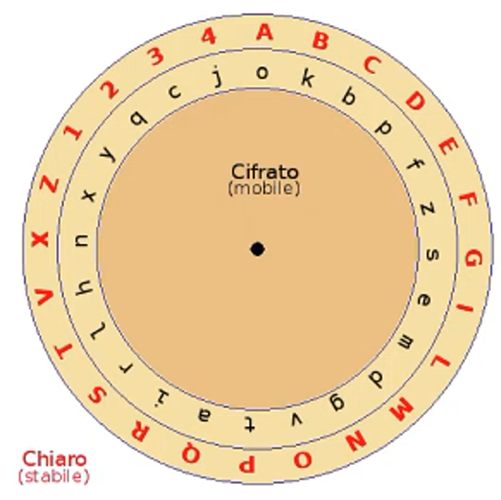
\includegraphics[scale=.45]{images/8.PNG}
\end{center}
\subsection{Primo metodo di cifratura} I dischi sono disposti in modo da ottenere la corrispondenza seguente...
\begin{verbatim}
ABCDEFGHILMNOPQRSTUVZ12345 <-- CHIAVE A-S
SDTKBJOHRZCUNYEPXVFWAGQILM

ABCDEFGHILMNOPQRSTUVZ12345 <-- CHIAVE A-Q
QILMSDTKBJOHRZCUNYEPXVFWAG

Chiave iniziale: A-S
messaggio: NON FIDARTI DI EVE
m = NONFIDA 2 RTIDIEVE
c = UNUJRKS Q UYBMBSPS
quando si arriva su 2 la chiave diventa A-Q
\end{verbatim}
Inizialmente abbiamo la chiave A-S, cioè indichiamo che tra i due dischi si debba avere corrispondenza tra A esterno ed S interno. Il numero due costituisce un carattere speciale, che determina un cambio di chiave: quando si arriva alla lettera Q si nota la corrispondenza con 2 e la chiave diventa A-Q (primo carattere con cui stabilisco la corrispondenza è sempre $A$, il secondo è quello che si trova nella corrispondenza con $2$).

\subsection{Secondo metodo di cifratura} C'è un secondo modo per usare questi dischi: il metodo dell' \emph{indice mobile}:
\begin{verbatim}
ABCDEFGHILMNOPQRSTUVZ12345 <-- CHIAVE A-E
EQHCWLMVPDNXAOGYIBZRJTSKUF

ABCDEFGHILMNOPQRSTUVZ12345 <-- CHIAVE A-P
PDNXAOGYIBZRJTSKUFEQHCWLMV

m: ILD 2 EL P FINO
c: PDC S WD O OIRJ
\end{verbatim}
Inizialmente la chiave è A-E, poi decifrando si trova 2: tra due lettere si cambia chiave. Si decifrano quindi altre 2 lettere nella giusta maniera e la lettera dopo sarà P cioè la nuova chiave A-P e successivamente si inizia a decifrare con questa nuova chiave. In genere si cambia chiave ogni volta che si trova un carattere speciale. Con caratteri speciali frequenti il cifrario è difficle da attaccare, poichè la chiave viene alterata ad intervalli imprevedibili.
\clearpage 

\section{Cifrario polialfabetico: De Vigenère}
\begin{framed}
\noindent \textbf{Esercizio da esame}.\\
Esporre come funziona il cifrario di de Vigenère e descrivere il principale attacco che può essere
condotto contro di esso.
\end{framed} 
E' una estensione della tecnica dell'Alberti più sicura che è rimasta irrompibile per 3 secoli. Si sceglie una chiave in cui ogni lettera corrisponde ad un numero che sarà di quanto bisogna shiftare il testo in chiaro per ottenere il testo cifrato:
\begin{table}[ht!]
    \centering
    \begin{tabular}{c c c c c c}
        C & H & I & A & V & E \\
        2 & 7 & 8 & 0 & 24 & 4
    \end{tabular}
\end{table}
la chiave si ripete tante volte quanto serve per equiparare il messaggio in lunghezza (nel caso in cui la lunghezza della chiave sia più piccola del messaggio da cifrare):
\begin{center}
	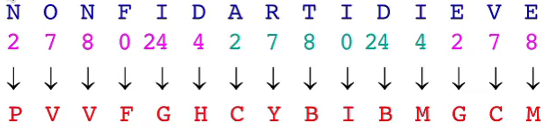
\includegraphics{images/9.PNG}
\end{center}

\paragraph{Rappresentazione alternativa con matrice} Si può vedere anche con una matrice 26x26 in cui ad ogni incrocio si trova la lettera $i$ criptata con la lettera $j$. In sostanza indichiamo nella matrice non i numeri rappresentanti le traslazioni, ma direttamente i caratteri.

\paragraph{Sicurezza della chiave} La sicurezza di questo metodo è influenzata dalla lunghezza della chiave: se la chiave è di piccola dimensione allora il numero di volte in cui si manifestano certa traslazioni aumenta. Addirittura, ponendo la chiave con dimensione $h=1$ ottengo l'equivalente del cifrario monoalfabetico di Cesare. Maggiore è la lunghezza della chiave, maggiore è la sicurezza.
\begin{itemize}
	\item \textbf{Idea di attacco}.
	
	Supponiamo di conoscere la lunghezza $h$ della chiave; costruiamo dei sottomessaggi formati dalle lettere che occupano tutte le stesse posizioni mod $h$. In ciascuno di questi messaggi tutte le lettere sono allineate alla stessa lettera della chiave quindi è come se fossero cifrate con un metodo monoalfabetico.
	
	\item \textbf{Sicurezza a confronto coi cifrari monoalfabetici}.
	
	I cifrari polialfabetici non sono molto più sicuri dei metodi monoalfabetici se le chiavi sono piccole! Se la chiave è lunga quanto il messaggio, è casuale e non riutilizzata otteniamo un cifrario \emph{perfetto} (ovviamente aumenta la difficoltà d'uso). E' il caso del \emph{one-time-pad} che usa una codifica binaria (1917).
\end{itemize}
\clearpage 

\chapter{Cifrari a trasposizione}
In questi cifrari non sostituiamo lettere come fatto fino ad ora. Il crittogramma presenta le seguenti caratteristica:
\begin{itemize}
	\item è una permutazione dei caratteri del mess aggio originario;
	\item in alcuni casi può includere lettere aggiuntive, ignorate nella decifrazione.
\end{itemize}

\section{Cifrario a permutazione semplice} 
La chiave consiste nella coppia $<h, \Pi>$. 
\begin{itemize}
	\item Dividiamo il messaggio da cifrare in blocchi aventi lunghezza $h$. Nel caso in cui il numero di caratteri che costituiscono il messaggio non sia multiplo di $h$ andremo ad aggiungere nell'ultimo blocco dei \emph{caratteri padding}, in modo che tutti i blocchi siano di dimensione $h$.
	\item Definiamo un insieme di posizioni $\Pi$, con cui rappresento una permutazione degli interi $\{1,\dots,h\}$ (ovviamente ho un numero di interi pari a $h$).
\end{itemize}
Vediamo col seguente esempio.
\paragraph{Esempio} $h = 9, \Pi=\{1, 2, 5, 3, 7, 6, 4, 9, 8\}$
\begin{center}
	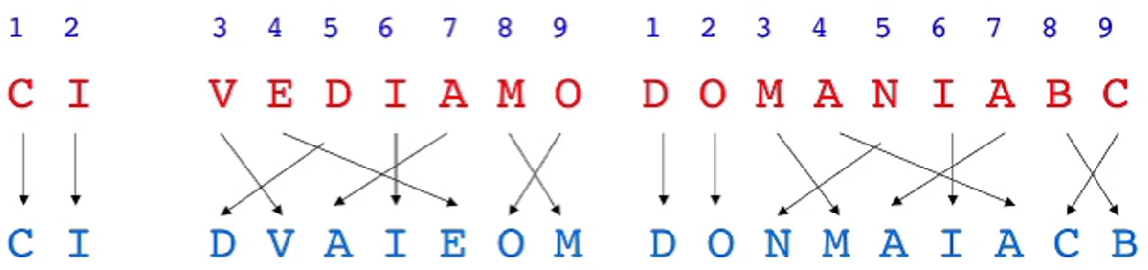
\includegraphics[scale=.5]{images/10.PNG}
\end{center}
\paragraph{Numero di chiavi possibili} Le chiavi sono le possibili permutazioni: $h!-1$. Non si considera quella che lascia invariato il messaggio.
\section{Cifrario a permutazione di colonne}
La chiave consiste nella terna $k=<c, r, \Pi>$
\begin{itemize}
	\item $c$ ed $r$ sono il numero di colonne e righe di un tavolo da lavoro $T$ dove andremo a collocare il messaggio in chiaro (di fatto il tavolo da lavoro è una matrice di $r$ righe e $c$ colonne).
	\item $\Pi$ è la permutazione degli elementi $\{1, 2, \dots, c\}$. Ciò che andremo a spostare non sono caratteri, ma colonne del tavolo $T$!
\end{itemize}
Si prende il messaggio e lo si decompone in blocchi $m_1, m_2, \dots$ di $c \times r$ caratteri ciascuno, eventualmente aggiungendo \textit{padding}. I caratteri si distribuiscono tra le celle della matrice $T$, riempiendo le righe dall'alto verso il basso. Si veda il seguente esempio.

\paragraph{Esempio} Vogliamo cifrare la frase \emph{NON SONO IL COLPEVOLE}.
$$c = 6, r = 3, \Pi=\{2, 1, 5, 3, 4, 6\}$$
\begin{center}
	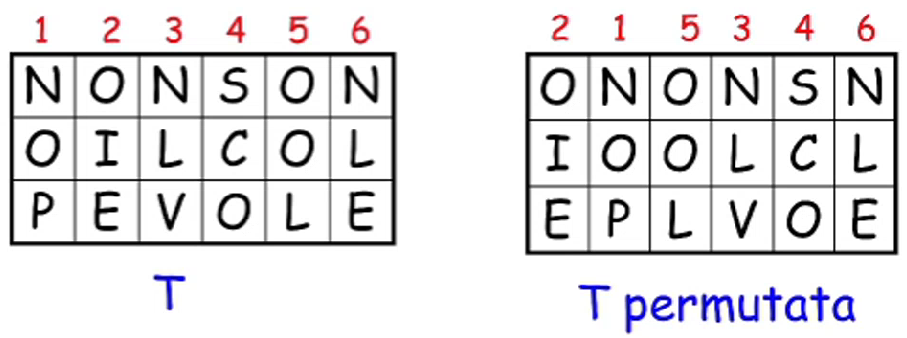
\includegraphics[scale=.4]{images/11.PNG}
\end{center}
Dalla lettura per colonne otteniamo il crittogramma \textit{OIENOPOOLNLVSCONLE}. In questo caso facciamo tutto in un unico blocco. Le chiavi sono esponenziali non avendo un tetto massimo per $r$ e $c$.


\section{Cifrario a griglia (\emph{cifrario di Richelieu})}
\begin{framed}
	\noindent \textbf{Domanda da esame}.\\Spiegare cosa s’intende per cifrario (storico) a griglia, indicare come si costruisce una griglia e
	quante griglie diverse si possono costruire per ogni dimensione scelta.
\end{framed} 
\paragraph{Versione innocente}
Un esempio è il cifrario di \emph{Richeliu}: il crittogramma è celato in un libro, la chiave è una scheda perforata e la pagina di un libro. Facendo corrispondere la scheda con la pagina si vedono le lettere che compongono il messaggio. Il fatto che si prenda la pagina di un libro garantisce il rispetto del principio di innocenza di Bacone. 
\paragraph{Versione non innocente} Rinunciando al principio di innocenza usiamo una griglia quadrata $q\times q$ con $q$ pari, $s = \frac{q^2}{4}$ è il numero delle celle trasparenti che compongono il messaggio. Si scrivono i primi $s$ caratteri del messaggio nelle posizioni corrispondenti alle celle trasparenti. La griglia viene ruotata tre volte di $90$° in senso orario e si ripete per ogni rotazione l'operazione di scrittura dei 3 gruppi successivi si $s$ caratteri.

\paragraph{Esempio} Vogliamo cifrare la frase \emph{L'ASSASSINO E' ARCHIMEDES TARRINGTON}.
\begin{center}
	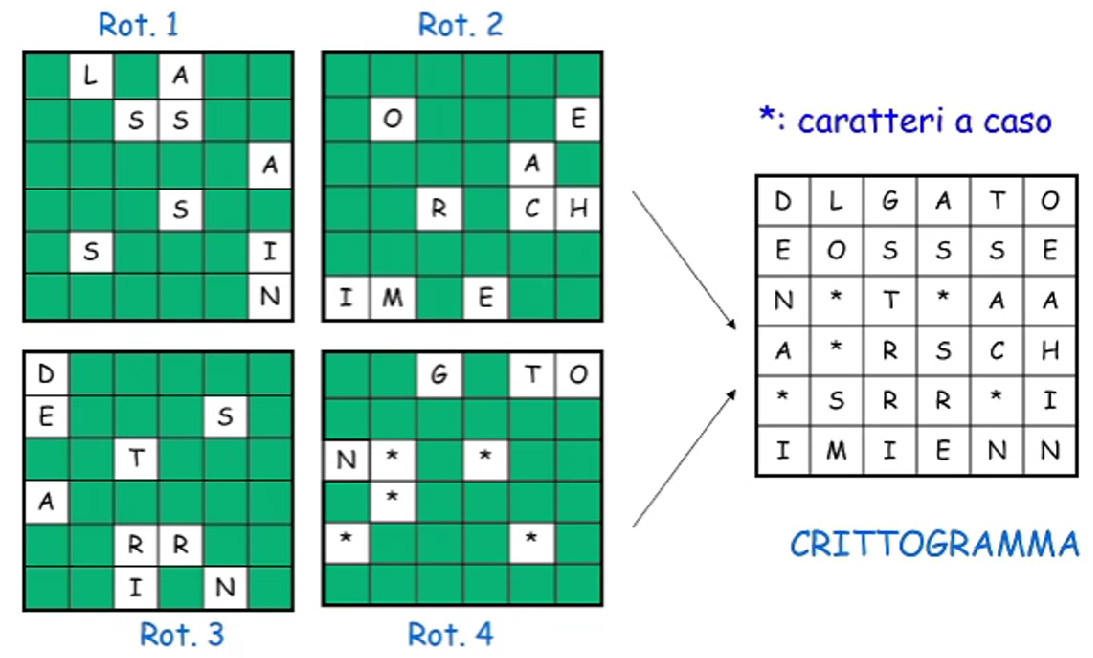
\includegraphics[scale=.38]{images/12.PNG}
\end{center}
Abbiamo $q=6, s=\frac{6^2}{4}=9$. La griglia va costruita in modo che una cella già usata non ricapiti nuovamente. Se la lunghezza è maggiore di $4s$ si riempiono più tabelle. La decifrazione si ottiene applicando la maschera e leggendo. 

\paragraph{Griglie possibili} Le griglie possibili sono $G = 4^s = 4^{\frac{q^2}{4}}$. Per $q=6$ otteniamo
$$G = 4^9 \approx 260'000$$Si arriva a questo numero perché:
\begin{itemize}
    \item immaginiamo di dover creare la maschera, scegliamo il primo foro e dobbiamo sceglierlo in modo che ruotando la griglia non sia nuovamente scoperto.
    \item si devono scegliere $s$ buchi, per ogni cella se ne deve scegliere una su 4 quindi $4^s$ chiavi possibili
\end{itemize}
\clearpage 

\chapter{Forzatura dei cifrari storici}
\section{Crittoanalisi statistica}
\begin{framed}
	\noindent \textbf{Domanda da esame}.\\Spiegare cosa s’intende per crittoanalisi statistica e come essa possa essere impiegata nell’attacco ai
	cifrari a sostituzione monoalfabetica e polialfabetica.
\end{framed} 
Abbiamo detto che la sicurezza di un cifrario dipende dalla dimensione delle chiavi, in modo tale da impedire la forzatura del cifrario stesso attraverso ricerche esaustive. Fino ad ora abbiamo pensato a forzature del cifrario con individuazione di chiave, ma il metodo non è l'unico possibile.  I cifrari storici, in particolare, sono stati violati con un attacco statistico di tipo \emph{cipher-text} (si conosce solo il crittogramma). 
\paragraph{Ipotesi} Il metodo si afferma in Europa nel XIX secolo con la forzatura del cifrario di Vigenère. Si fanno delle ipotesi:
\begin{itemize}
    \item si suppone di conoscere il metodo di cifratura/decifratura (si da per scontato che il crittoanalista conosca il metodo);
    \item si suppone che il crittoanalista conosca il messaggio naturale in cui sono scritti i messaggi;
    \item si suppone di avere messaggi abbastanza lunghi da far valere le statistiche note dei linguaggi naturali.
\end{itemize}
\begin{center}
	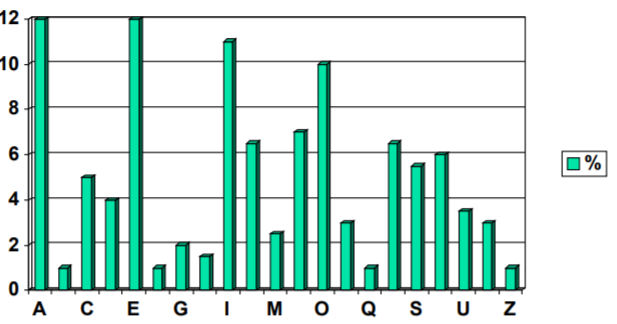
\includegraphics[scale=.56]{images/13.PNG}
\end{center}
La frequenza con cui appaiono le lettere dell'alfabeto è ben studiata in ogni lingua così come sono note le frequenze dei \emph{digrammi}, \emph{trigrammi}, \emph{q-grammi} (gruppi da 2, 3, $q$ lettere). Nell'italiano le lettere A ed E costituiscono il 12\% dei messaggi. Si calcola il grafico delle frequenze dei caratteri all'interno del crittogramma: se siamo davanti ad un cifrario a sostituzione monoalfabetico avremo un grafico che è permutazione del grafico delle frequenze italiane, possiamo quindi dire che è molto probabile che se $$\text{freq}\left(x\right) \approx \text{freq}\left(y\right)$$ allora $x$ è stato criptato con $y$.
%\paragraph{Istogramma delle frequenze} In genere l'istogramma delle frequenze è utile per individuare la tipologia di cifrario adottato.
%\begin{itemize}
%	\item \textbf{Trasposizione}: grafico pressochè identico a quello del linguaggio
%	\item \textbf{Sostituzione monoalfabetica}: permutazione del grafico del linguaggio
%	\item \textbf{Sostituzione polialfabetica}: grafico è pressoché piatto
%\end{itemize}
\section{Cifrari a sostituzione monoalfabetici}
\begin{itemize}
	\item \textbf{Cifrario di Cesare}. 
	
	Nel caso del cifrario di Cesare abbiamo uno shift del grafico. Ci basta individuare una corrispondenza per trovare tutte le altre. 
	
	\begin{center}
		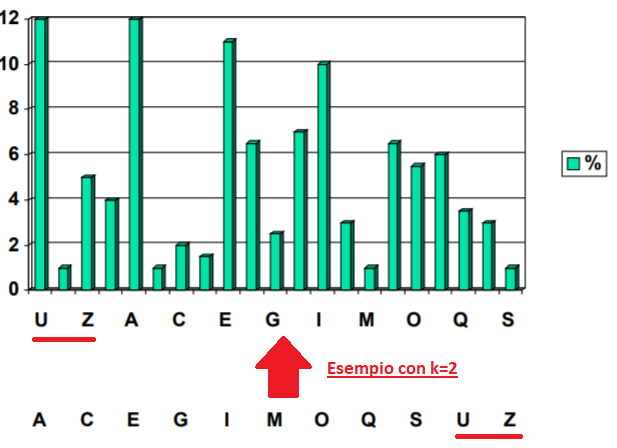
\includegraphics[scale=.55]{images/13bis.PNG}
	\end{center}

	L'attacco a forza bruta rimane la cosa più semplice, visto l'esiguo numero di chiavi. 
	
	\item \textbf{Cifrario affine}. 
	
	Nel caso di cifrari affini una volta trovate due lettere $a,b$ si imposta il sistema di equazioni e si risolve. Il cifrario è per definizione invertibile (basata avere $\text{MCD}(a,m)=1$, quindi $a,m$ coprimi), dunque la risoluzione del sistema è sempre possibile.
	\item \textbf{Cifrario completo}. 
	
	Nel caso di un cifrario completo (permutazione arbitraria) non abbiamo lo shift del grafico, ma una permutazione dove le frequenze non sono associate ai relativi caratteri. Quello che facciamo è associare le lettere del messaggio cifrato (l'unico che abbiamo) in base alle frequenze.
	
	\textbf{Esempio}: so che una lettera (o un insieme di lettere) è quella maggiormente utilizzata nella lingua italiana. Verifico nel cifrario quale carattere è stato utilizzato maggiormente: confrontando le frequenze potrei individuare una corrispondenza.
\end{itemize}
\clearpage 

\section{Cifrari a sostituzione polialfabetica} 
Nella sostituzione polialfabetica la decifrazione è più difficile! A una lettera possono corrispondere lettere diverse: l'istogramma delle frequenze è piatto.
\begin{itemize}
	\item \textbf{Cifrario dell'alberti}.
	
	Il cifrario dell'Alberti è immune da questi attacchi se la chiave viene cambiata spesso evitando \textit{pattern} ripetitivi. Mantenere la stessa chiave a lungo è come usare un cifrario monoalfabetico, precisamente un cifrario completo.
	
	\item \textbf{Cifrario di Vigenère}.
	\begin{itemize}
		\item La lettera $y$ non dipende solo dalla lettera del testo in chiaro, ma anche dalla lettera corrispondente della chiave.
		\item La chiave è spesso piccola e ripetuta più volte: se sappiamo che la chiave ha lunghezza $h$ possiamo raggruppare le lettere in posizioni $h,2h,3h,\dots$ e poi $h+1,2h+1,\dots$ e così via. In questo modo si ottengono $h$ gruppi cifrati in maniera monoalfabetica: se individuo una coppia allora individuo tutte le altre coppie del gruppo analizzato.
		\item Si deve stimare la lunghezza della chiave: si studiano i digrammi ed i trigrammi alla ricerca di sequenze che si ripetono nella speranza che lo stesso digramma/trigramma sia criptato allo stesso modo e si prende la loro distanza come multiplo della lunghezza della chiave (o la chiave stessa). E' molto più probabile che si generi in questo modo piuttosto che sia generato casualmente.
	\end{itemize}
\end{itemize}
\section{Cifrari a trasposizione}
Nei cifrari a trasposizione non ha senso calcolare l'istogramma delle frequenze in quanto il crittogramma è una permutazione delle lettere del testo in chiaro (le frequenze sono le stesse). In questi casi si usa lo studio dei q-grammi. In particolare se si sa la lunghezza $h$ della chiave:
\begin{itemize}
	\item si divide il crittogramma in blocchi di $h$ lettere
	\item in ciascun gruppo si cercano i gruppi di q lettere che formano i q-grammi più diffusi nel linguaggio
	\item se si trova un vero q-gramma si ottiene parte della chiave
\end{itemize}

\begin{framed}
	\noindent \textbf{Osservazione conclusiva}. 
	
	\noindent La crittoanalisi statistica permette di fare due cose:
	\begin{itemize}
		\item individuare il possibile cifrario adottato da chi ha generato il crittogramma;
		\item individuare (in alcuni casi) le corrispondenze, cioè decifrare in tutto o in parte il crittogramma.
	\end{itemize}
\end{framed} 

\chapter{La macchina Enigma}
Rappresenta l'ultimo esempio di cifrario storico, il primo che porta a dei sistemi automatizzati e gli sforzi fatti per rompere questo sistema sono stati importanti per l'evoluzione storica dell'informatica. Nasce in Germania nel 1918 ed è una modifica automatizzata del cifrario dell'Alberti.
\begin{center}
	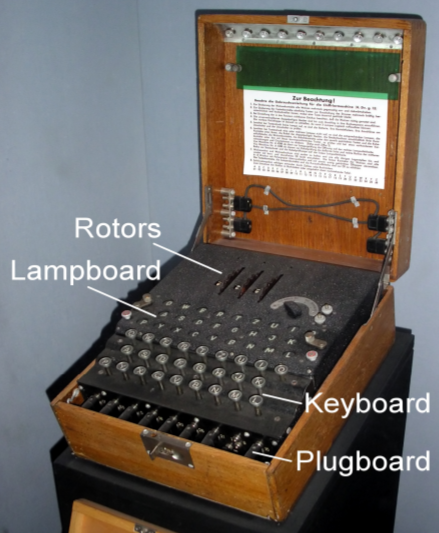
\includegraphics[scale=.55]{images/14.PNG}
\end{center}
Si compone di una tastiera di ventisei lettere (alfabeto tedesco) più altrettante lampadine rappresentanti lettere. Ogni volta che l'utente preme un tasto si illumina il corrispondente carattere del crittogramma. L'utente osserva la luce accesa, si segna la lettera e prosegue col carattere successivo. Lo stesso approccio vale per la decifrazione. Si osservi che nella cifratura premere più volte lo stesso carattere sulla tastiera porta ad ottenere un crittogramma costituito da caratteri diversi.
\section{Chiave e assetto iniziale} La chiave è l'assetto iniziale della macchina. Questo assetto rende reversibile la cifratura: un assetto permette di cifrare ($A \xrightarrow{} F$) ma anche di decifrare ($F \xrightarrow{} A$). Ciascun interlocutore presenta una macchina enigma: affinchè il destinatario possa decifrare un messaggio è necessario che tutti gli interlocutori abbiano lo stesso assetto iniziale.

\section{Interno della macchina} All'interno abbiamo un \emph{riflettore} e \emph{3 rotori} (dischi in grado di ruotare in modo indipendente). 
\begin{center}
	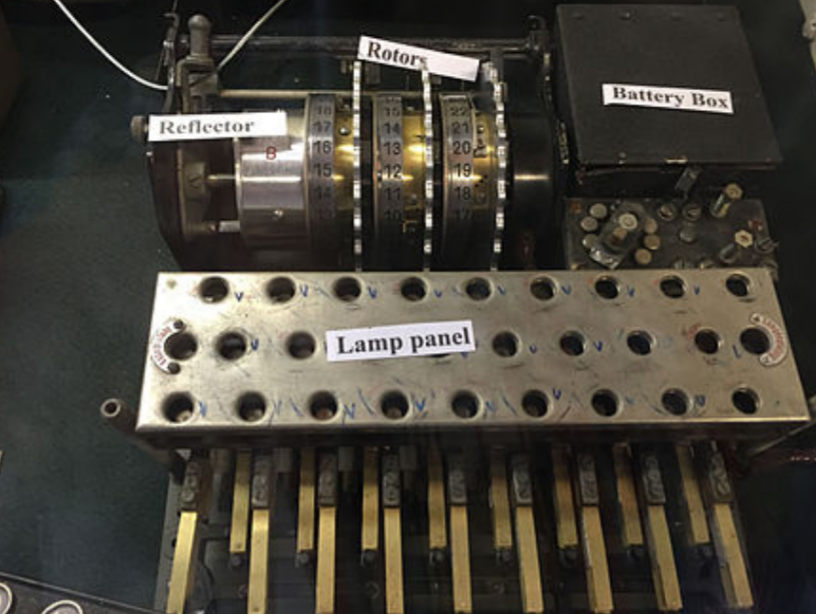
\includegraphics[scale=.4]{images/15.PNG}
	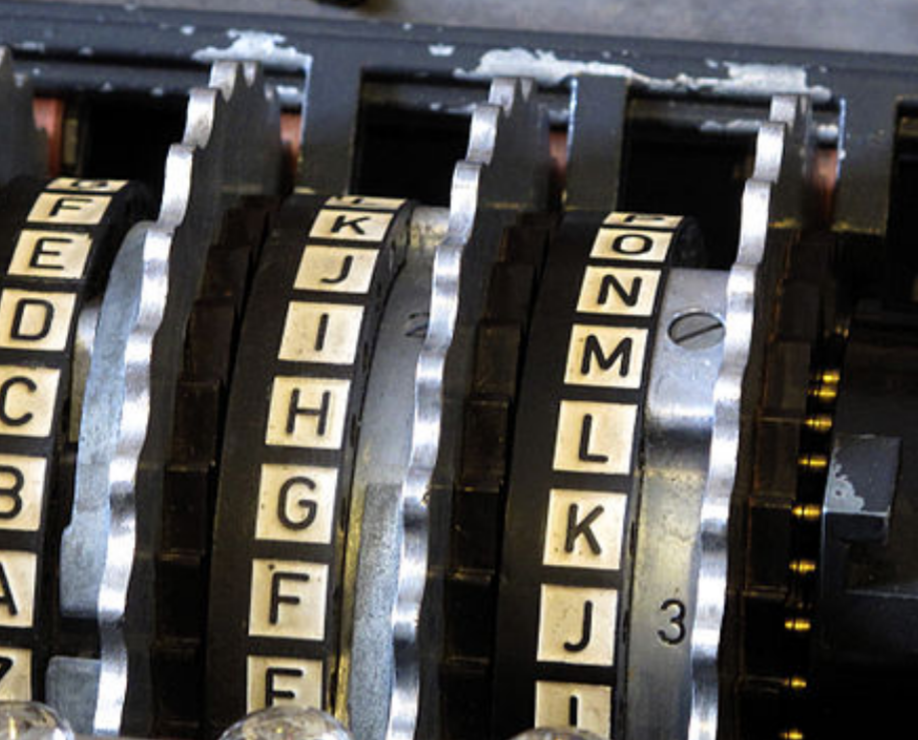
\includegraphics[scale=.33]{images/16.PNG}
\end{center}
Il riflettore è anch'esso un rotore modificato. Per aumentare lo spazio delle chiavi si aggiunge una \emph{plugboard} cioè una batteria di connettori che mette in corrispondenza diretta due lettere (in un certo senso è come se scambiassi di posizione due lettere, premo una e in realtà ne sto premendo un'altra). 
\begin{center}
	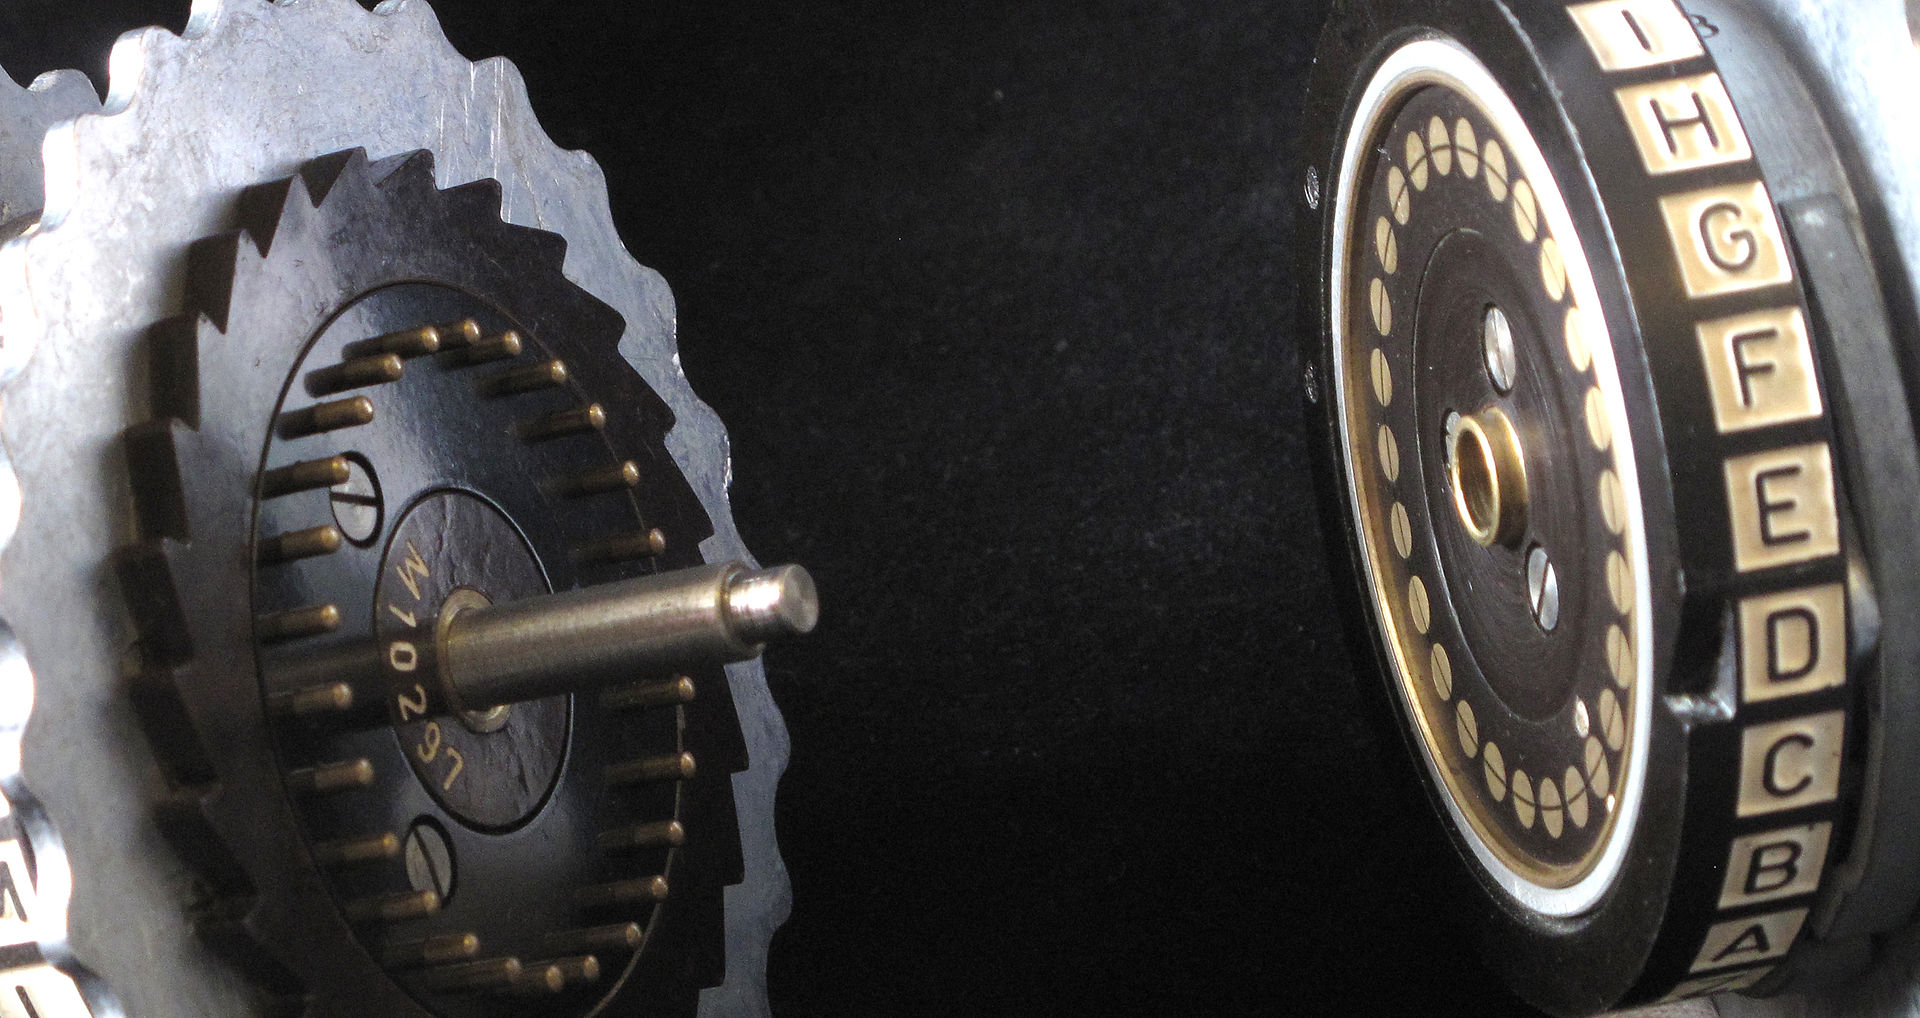
\includegraphics[scale=.35]{images/17.jpg}
\end{center}
Ogni rotore rappresenta la permutazione di un alfabeto. Possiede due facce : \emph{pad} e \emph{pin}, ciascuna con ventisei contatti elettrici disposti in cerchio e ciascuno associato a una particolare lettera. Si ha un cablaggio fisso che collega i contatti di una faccia con quelli di un'altra.
\begin{center}
  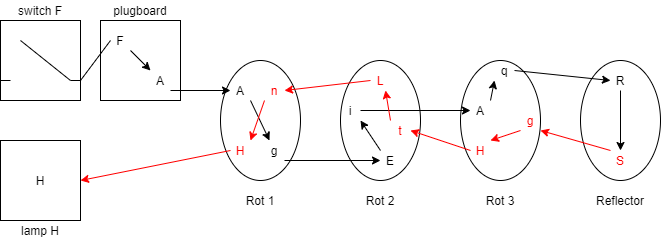
\includegraphics[width = 350pt]{images/Enigma.png}
\end{center}

\begin{itemize}
	\item Per costruzione una lettera non è mai cifrata con se stessa. Questa proprietà e quella di riflessione sono state utilissime nel rompere questo sistema.
	\item I rotori non sono fissi.
	\begin{itemize}
		\item Il primo rotore avanza di un passo per ogni lettera battuta sulla tastiera.
		\item Dopo 26 passi il primo rotore torna sulla posizione iniziale, quindi si muove di una posizione il secondo rotore.
		\item Dopo la rotazione completa del secondo rotore si muove di un passo il terzo rotore.
	\end{itemize}
	Questa cosa comporta una chiave cambiata ad ogni passo.
	\item Le permutazioni sono 26 per il primo rotore rispetto al secondo, 26 del secondo rispetto al terzo, 26 del terzo rispetto al riflettore: $$26 \cdot 26 \cdot 26 = 17.576$$ chiavi se i rotori sono immutabili e noti a chiunque ne avesse una copia. 
	\item Si aumentano le chiavi scambiando l'ordine dei rotori, quindi si sale a ${26}^3 \cdot \left(3!\right) > 10^5$.
	\item Aggiungendo le plugboard si possono scambiare 6 coppie di caratteri per ogni trasmissione, si arriva quindi ad una sequenza di 12 caratteri per descrivere il cablaggio: le combinazioni possibili sono $$\binom{26}{12} \approx 10^7$$ Scelte le lettere va scelta la loro ordinazione: 
	$$\binom{26}{12} \cdot 12!$$
	In realtà dobbiamo escludere delle permutazioni, quelle che lasciano lo stesso effetto, quindi dividiamo per $6!$ e per $2^6$
	\begin{center}
		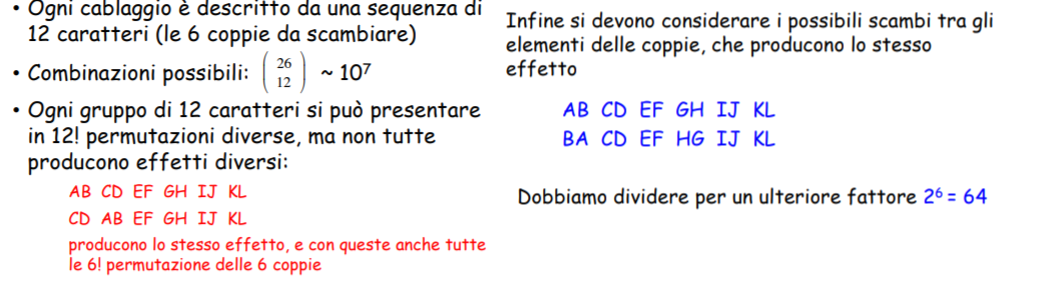
\includegraphics[scale=.75]{images/26.PNG}
	\end{center}
\end{itemize}
